\chapter{Correctness proofs}
\label{cpt:correct}

%\jf{Add some pieces of Coq and LTac code}
In this chapter we introduce the correctness proofs we have performed
for the ARMv6 instruction set simulator \simlight by using the operational semantics
of \compcert C.
This work can be also considered as a significant experiment on
proving C programs by using a formalized operational semantics of C.

\selectlanguage{french}
\section*{Résumé}

\begin{resume}
Ce chapitre est consacré aux preuves de correction que nous avons effectuées
pour \simlight, le simulateur de jeu d'instructions de l'ARMv6 de notre projet,
en utilisant la sémantique opérationnelle de \compcert C.
Ce travail peut également être considéré comme une expérience significative
de preuves de programmes C selon une approche basée sur la sémantique opérationnelle.

Essentiellement, nous avons à établir qu'un programme C représentant l'ARMv6
se comporte conformément au modèle Coq attendu,
qui est un système de transitions sur un état abstrait directment défini en Coq.
Le programme C, via la sémantique opérationnelle définie dans \compcert,
est lui même modélisé par un système de transitions sur un état en un sens plus concret,
qui est un modèle de la mémoire C (telle qu'elle est formalisée dans \compcert),
habitée par des structures de données indiquées dans le programme \simlight.
Bien que le programme C et le modèle Coq soient dérivés à partir des mêmes
données du manuel de référence, et que la chaîne de génération de ces deux objets
soit en partie partagée,
on voit que ces objets sont de nature très différente.
Le modèle Coq abstrait reste aussi simple que possible
de façon à respecter visiblement ce qui est énoncé dans le manuel de référence.
En revanche, l'état concret pour \simlight prend non seulement en compte
le modèle mémoire de \compcert C,
mais des structures de données C complexifiées par un souci d'optimisation.

Afin de comparer le comportement du système de transition abstrait dans le modèle Coq
et celui du système de transition concret correspondant à \simlight,
nous commençons par définir une projection de l'état concret verts l'état abstrait.
Nous pouvons alors énoncer, pour chaque instruction ARM,
un théorème principal schématise en figure~\ref{fig:theo}
(une version plus exacte est donnée plus loin en figure~\ref{fig:theoca}).

Le preuves s'effectuent alors en itérant l'analyse des hypothèses
représentant des transitions entre états mémoire concrets,
selon une relation appropriée de la sémantique opérationnelle à grand pas
de \compcert C.
La transition correspondant dans le modèle abstrait est représentée
plus simplement par calcul,
car dans le modèle Coq de l'ARMv6, les instructions sont représentées par des fonctions.
\end{resume}

\selectlanguage{english}

\section{General idea}
\label{sec:gi}

% \margxm{1}{Consider the work as the proof for simulator and the proof for general C code}

% JF->XM: "C specification" is improper. Use "C program" or "C implementation"

% % XM
% For the ARMv6 ISS model, we build a Coq model on one hand,
% on the other, we have a C model from the same ARMv6 AST representation
%
% % JF
For the ARMv6 Instruction Set Simulator \simlight,
we have to compare a Coq model with a C implementation
(see Section~\ref{sec:overall}).

% % XM
% The correctness proofs will be processed in Coq proof system.  But how
% to deal with two models in two languages.  \compcert helps to build a
% bridge between them.  The general idea is to use the \compcert defined
% C formal syntax and semantics, which are specialized in Coq
% system. From it, we can obtain again a C model in Coq again.  With these two
% representations in Coq, it is able to begin the correctness proof.
%
% % JF
In order to formally reason on the correctness of the second with relation to the first
in the Coq setting,
we need a formal model in Coq of the C implementation.
It is provided by \compcert,
which defines a operational semantics of C formalized in Coq.
The two Coq models to be compared are state transition systems.

% % XM
% Although these two representations come from the same AST, the results are quite
% isolated from each other.
% From the macro point of view, the Coq specification follows exactly ARMv6
% reference manual, and keeps everything as simple as possible.
% The C specification has more objectives to achieve
% because \simsoc is aimed to be a high speed simulator.
% So optimization and some complex type definitions are required during the model
% design phase.
%
% % JF
Note that a large part of these two models is automatically derived
from the same source,
that is, an AST representation of the pseudo-code for instructions
taken in the ARMv6 manual.
However, even for this part, it is far from obvious that the two models
behave the same.
They are actually quite different from each other.  % JF isolated -> different

Basically,
the Coq specification follows exactly ARMv6 reference manual,
and keeps everything as simple as possible.
whereas the C program has more objectives to achieve
because it is aimed to be a high speed simulator.
In particular,
states in the model of the C implementation are much more complex
not only because the memory model defined in \compcert is taken into account,
but also because of optimizations and design decisions in \simlight
targetting efficiency.
In more detail:
\begin{itemize}
\item
% % XM
% The different type system.
% % JF No, a type system is something else. You mean data types. Ask me next time
The C implementation uses a big \emph{struct} to express the
ARM processor state.
The model of the state is a complex Coq record type, including not only data fields
but also proofs to guaranteed access permission, next block pointer, etc.
This is detailed in Section~\ref{sec:proj}.
\item
In the Coq specification,
% % XM
% semantics is in definition
% %  JF
transitions are defined in a functional style,
whereas in the model of the C implementation, a relational style is used.
%\margjf{1}{I added some ideas here}%
In general, the relational style is more flexible but
functional definitions have some advantages:
reasoning steps can be replaced by computations;
existence and unicity of the result are automatically ensured.
However, the functional style is not always convenient or even possible.
It is the case here, where the transitions defined by the C implementation
are relations which happen to be functions.
This comes first from the operational semantics, which needs to be relation
for the sake of generality.
Furthermore in our case,
the kind of record type mentioned in the previous item
is too complex to execute calculation with it,
so it is
more convenient to describe the state transformation for memory with a relation.
%
% because it is the semantics designed just for our instruction simulation.
% And in this simplified simulator, it does not implement co-processor or other
% features to interrupt the instruction operation.
% After one instruction, the processor will always turn to a new state.
% Whereas \compcert defines the semantics for C language, it is
% % % XM
% % in relation.
% % %  JF -- anyway commented out and rewrote the whole parag
% defined in a relational style,
% That is because the compiler translation line is certified by proving the same behavior
% of input and output languages. This \textbf{behavior} is expressed by program
% termination.
%
% The following is moved ot the previous item
% And the memory state is a complex Coq record type, including not only data field
% but also proofs to guaranteed access permission, next block pointer, etc.
% This kind of record type is too complex to execute calculation with it, so it is
% more convenient to have relation to describe the state transformation for memory.
\item
The two semantics operates on very different states.
For the Coq specification,
reading or changing the value of the processor state or other related variables
is easy to express.
In the model of the program, the state is based on a complex memory model
and load and store functions are used for read/write operations%\margjf{1}{to be checked by XM}.
% % XM original
% Two semantics operates on different memory systems.
% For Coq specification, semantics directly operates on processor state and
% other related variables. The value of these variables can be easily read or
% changed. However, the C semantics is based on the model of a whole memory used by
% compiler.
% The semantics, such as evaluation of statements and expressions,
% is described by a relation between initial and final memory state.
% Then, to get value of processor state or any variable, we need to load and store
% from memory state model.
\end{itemize}

\begin{figure}
\hfil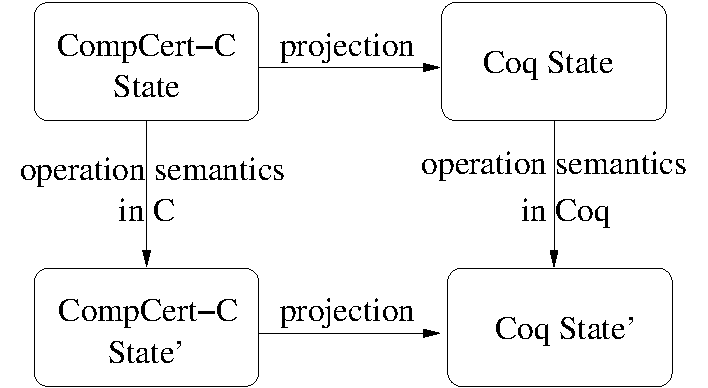
\includegraphics[width=.75\linewidth]{fig/theorem.pdf}

\caption{Main theorem for a given ARM instruction}
\label{fig:theo}
\end{figure}

For a given operation,
we state and proof
a main theorem which can be displayed by the diagram in Figure~\ref{fig:theo}.
On both sides, the execution of an instruction is described by a state transition.
% % XM (removed by JF, contents-free)
% From executing one instruction, the processor state will turn into
% a new state.
For the two ISS representations, ``State'' refers to the full description of
the system.
We start from a C memory state corresponding to
a more abstract state described by the Coq specification.
This correspondance is expressed by a projection relating the two models
of the state.
Then, executing the same instruction
on two sides will produce a pair of new processor states
which are related by the same correspondance.
Informally,
executing the same instruction on a pair equivalent states
will produce a pair of equivalent states.
%
% % XM Original
% if we have a pair of equivalent processor state, executing the same instruction
% on two sides will produce a pair of new processor state, which are equivalent
% again.
% Then we say, the C model has an instruction operates exactly like the
% formal model, and it is proved correct.

% \subsection{\compcert library}

% The \compcert library can be discussed in two parts.
% First is a collection for often used operation in Coq definitions and proofs.
% There are definitions and theorems about type \texttt{positive}, \texttt{Z},
% \texttt{nat} and conversion among them. Definitions and proofs on option
% type, list, boolean and etc.
% The second is the definitions on machine integers, and bitwise operations.
% It is based on Coq integer \texttt{Z}, and a proof to guaranteed the value is under
% the range from 0 to modulus.
% This module also support the conversion between type \texttt{Z}, \texttt{int} and
% \texttt{nat}.
% This can be extend to integers of size 8, 32 and 64 bits in our \emph{Bitvec}
% file.

% In \compcert, applicative finite maps are the main data structure used in
% memory state, global/local environment descriptions.
% There are two basic type, a \coqdocvar{Tree} and a \coqdocvar{Map},
% from them a number of maps and trees can be derived.
% The difference between the two is:
% For \coqdocvar{Tree} the return of $\langle get\rangle$ operation is an option type, if there is no
% data associated with key \coqdocvar{None} is returned. For \coqdocvar{Map} $\langle get\rangle$
% always returns data. If there is no data associated, a default value will be returned which is
% given since initialisation time.
% They two are both based on the abstract signature radix-2 search tree.
% And the derived trees and maps are named by their keys which can be integer or positive.
% The \coqdocvar{Tree} is used to define global and local environment which gathers memory
% information, maps the reference identifier to data information. Since the environment is built
% due to the memory contents, you can't get any information if you ask for a nonexistent address.
% On the contrary, memory content uses \coqdocvar{Map} indexed by integer. If a block
% in memory has not been allocated, it should return a default value \coqdocvar{Undefined} by
% any visit.

% %Applicative finite maps are the main data structure used in this
% %  project.  A finite map associates data to keys.  The two main operations
% %  are [set k d m], which returns a map identical to [m] except that [d]
% %  is associated to [k], and [get k m] which returns the data associated
% %  to key [k] in map [m].  In this library, we distinguish two kinds of maps:
% %- Trees: the [get] operation returns an option type, either [None]
% %  if no data is associated to the key, or [Some d] otherwise.
% %- Maps: the [get] operation always returns a data.  If no data was explicitly
% %  associated with the key, a default data provided at map initialisation time
% %  is returned.
% %
% %  In this library, we provide efficient implementations of trees and
% %  maps whose keys range over the type [positive] of binary positive
% %  integers or any type that can be injected into [positive].  The
% %  implementation is based on radix-2 search trees (uncompressed
% %  Patricia trees) and guarantees logarithmic-time operations.  An
% %  inefficient implementation of maps as functions is also provided.



% \subsection{\compcert C semantics}
% \label{sec:ccc}
% \compcert C is a large subset of C language.
% There are several things that is not supported by this subset.
% \begin{itemize}
% \item Types: it supports most of the types in C90 \cite{C90},
%   except the following points.
%   \begin{enumerate}
%   \item Unprototyped function type $(int f())$
%     and function type with variable number of arguments $(int f(...))$.
%     But it is possible to declare (not define) an external function of
%     the latter.
%   \item A structure can' have an unknown sized array type as the last
%     element. The size information must be known.
%   \end{enumerate}
% \item Wide char and wide string.
% \item Type cast do not support pointer to float.
% %\item The in-memory representation of pointer is opaque, can only be examined by
% %  a 32bits word.
% \item Specify bit fields in unions are not supported.
% \item In-line assembly is not supported.
% \item For the switch statement, \texttt{case} and \texttt{default} must appear.
%   And the \texttt{default} must occur at last.
% \item The only available external functions are printf, malloc, free,
%   \_\_builtin\_annot and \_\_bultin\_annot\_val. The other external functions can be
% declared but not implemented. One external function will generate a event trace.
% It says the result of the external function is computed by operating system,
% not the \compcert C code.
% \item Every program must has a \texttt{main} function declared.
% \end{itemize}


% When we want to obtain the \compcert C representation of ARMv6 model, there are
% two ways. First, use the \compcert C provide converter to generate \compcert
% C code from \simlight C file, this is not a verified translation step in \compcert.
% Or, we translate from the ARM internal representation
% AST to \compcert C AST.
% If we use the first method, the unsupported things above
% will not be controlled. The generated code may lose information without warning.
% So the second transformation is in use.
% The second transformation also has weakness. The ARM internal AST only contain the
% ISS model. The function body of library functions are not included.
% It means, the generated code has no definition of these library functions.
% We have to add them manually, or improve the feature of the transformation by
% invoking the former.
% Whichever transformation we choose, we have to give a fake main function.
% Because our correctness proof takes each instruction operation as one program.
% To build a \compcert C program, we must have the main entry point in the global
% environment.

% The semantics definition has two aspects. One is in small-step strategy,
% the other is in big-step.
% In our case, the big-step semantics is enough for correctness proofs.

% \compcert C describes C semantics in their memory model.
% Statement and expression evaluation is deterministic.
% The evaluation is represent using relation for a better proof induction.
% %%Coq had better support for proof induction over relations than over function definitions
% The formal operational semantics is described as transition system
% on memory states.
% $$G,E~\vdash ~\langle\textrm{expressions}\rangle,~M~\overset{t}{\Rightarrow}~v,~M'$$
% Here G represents global environment of whole program, E is the local environment,
% M and M' are memory states and t is a trace of I/O events,
% then v is a returned value.
% In \compcert C, expressions can be categoried into 15 cases and we have 13 of them
% are used in our correctness proofs.
% Some of the expressions are similar to the one for Clight and are already listed
% in \compcert papers \cite{lerbla08}.
% In Fig.~\ref{fig:evalexpr}, the inference rules different from Clight is showed.
% \begin{figure}
% \begin{minipage}[b]{1\linewidth}
% \centering
% %\small

% %  eval_call: forall e m rf rargs ty t1 m1 rf' t2 m2 rargs' vf vargs
% %                       targs tres fd t3 m3 vres,
% %       eval_expr e m RV rf t1 m1 rf' -> eval_exprlist e m1 rargs t2 m2 rargs' ->
% %       eval_simple_rvalue ge e m2 rf' vf ->
% %       eval_simple_list ge e m2 rargs' targs vargs ->
% %       classify_fun (typeof rf) = fun_case_f targs tres ->
% %       Genv.find_funct ge vf = Some fd ->
% %       type_of_fundef fd = Tfunction targs tres ->
% %       eval_funcall m2 fd vargs t3 m3 vres ->
% %       eval_expr e m RV (Ecall rf rargs ty) (t1**t2**t3) m3 (Eval vres ty)
% $$\frac
% {\begin{array}{c}
% G,E\vdash rf~M~\overset{t1}{\Rightarrow}~rf',M1\qquad
% G,E\vdash rarg^*~M1~\overset{t2}{\Rightarrow}~rarg'^*,M2\\
% G,E\vdash M2~rf' \Rightarrow vf\qquad
% \texttt{find\_funct}~(G,vf)~=~\lfloor fd\rfloor\\
% \vdash M2~fd~varg^* \overset{t3}{\Rightarrow}vres,M3
% \end{array}
% }
% {G,E\vdash M~\langle\textrm{\texttt{Call}}\rangle\overset{t1**t2**t3}{\Longrightarrow}vres,M3}
% $$
% \end{minipage}

% \begin{minipage}[b]{1\linewidth}
% \centering
%    % eval_assign: forall e m l r ty t1 m1 l' t2 m2 r' b ofs v v' t3 m3,
%    %    eval_expr e m LV l t1 m1 l' -> eval_expr e m1 RV r t2 m2 r' ->
%    %    eval_simple_lvalue ge e m2 l' b ofs ->
%    %    eval_simple_rvalue ge e m2 r' v ->
%    %    sem_cast v (typeof r) (typeof l) = Some v' ->
%    %    assign_loc ge (typeof l) m2 b ofs v' t3 m3 ->
%    %    ty = typeof l ->
%    %    eval_expr e m RV (Eassign l r ty) (t1**t2**t3) m3 (Eval v' ty)
% $$\frac
% {\begin{array}{c}
% G,E\vdash l~M\overset{t1}{\Rightarrow}l',M1\qquad
% G,E\vdash r~M1\overset{t2}{\Rightarrow}r',M2\\
% G,E\vdash l'~M2\Rightarrow (b, ofs)\qquad
% G,E\vdash r'~M2\Rightarrow v\\
% cast(v,typeof(l),typeof(r))=~\lfloor v'\rfloor\\
% store (G,~typeof(l),~M2,~(b,ofs),~v)=~\lfloor M3\rfloor\\
% \end{array}
% }
% {G,E\vdash (l=r)~M\overset{t1**t2**t3}{\Longrightarrow}v',M3}
% $$
% \end{minipage}
% \caption{Rules of operational semantics of \compcert C}
% \label{fig:evalexpr}
% \end{figure}


% The first rule in Fig~\ref{fig:evalexpr} is for evaluating function call
% expression. The evaluation is quite different from the rule for Clight.
% Not only that Clight is side-effect free, but \compcert C separates memory state
% transformation from evaluating simple expressions in order to preserve memory
% state.
% A function call can be evaluated in three steps:
% evaluating the function reference by identifier \coqdocvar{rf} to get where it
% stores;\\
% evaluating the function arguments references \coqdocvar{rargs} to get their
% values;\\
% finding the function definition \coqdocvar{fd} in the environment;
% then evaluating function call using \coqdocvar{eval\_funcall}.

% The second rule in Fig~\ref{fig:evalexpr} is evaluation of assignement expression.
% For Clight semantics, assignement is not an expression but a statement
% because Clight only accepts pure expressions.



\section{The ARMv6 model in \compcert C}
\label{sec:arm_ccc}


% % XM [JF: I don't understand what you say here]
% The top level of a \compcert C model is \texttt{program}.
% Program is defined as a record of \texttt{functions} (list of functions),
% the program entry point \texttt{main}, and (\texttt{global\_variables}).
% % JF [I write soemthing which makes sense but may be wrong,
% %     I don't know this detail about \compcert]
A \compcert C program a list of functions, including
the program entry point called \texttt{main},
with global variables as parameters.
% % JF: irrelevant
% We put each instruction pseudo-code in its own file.
The transformation from pseudo-code AST to \compcert C AST
% % XM
% will treat every instruction as a program itself.
% % JF
produces a standalone program for each ARMv6 instruction.
Then each has its own correctness proof separately.
In the generated \compcert C file, program contains only one function which is
the instruction operation. Other invoked functions are not included
because the instruction pseudo-code AST has nothing but a reference name.
% % XM
% In order to have these internal called function bodies, we have to add them
% manually into the functions list of the corresponding program.
% % JF
Their bodies are then manually included.

Every function is composed by its return type, function parameters,
local variables, and the function body.
The function body is a sequence of statements made of
expressions.
% % XM
% \compcert has very detailed syntax about every component.
% According expression definition,
% % JF
In \compcert ASTs, constructs are very detailed.
%
Each expression and each statement is annotated with its own type.
% In a program, the same definition of type may appear several times.
In a program, the same type may appear several times.
In the raw output of an AST, large and repeated expressions for types
occur everywhere,
making \compcert ASTs much more verbose and space consuming than necessary
and very hard to read.
In order to solve this issue and, more generally, get a readable code,
the pretty printer for ASTs introduces auxiliary names for types
-- common subtypes are then shared --
and also uses special notations for most constructs expression.
%\margjf{2}{I think that this was contributed by Fred B and Fred Tuong, no? Yes}
The implementation of this part was contributed by Frédéric Blanqui and Frédéric Tuong.

% Orig XM
% The raw output AST has the type defined every time when it was used.
% This made some long type definition repeat frequently and code looks messy.
% And printed code of \compcert C in Coq is too long and hard to read.
% In order to have a readable code,
% the pretty print code also uses special notations
% to denote each expression, and is optimized to define only once
% those sharing types.

% Definition fun_internal_B :=
%   {| fn_return := void;
%      fn_params := [
% proc -: `*` typ_SLv6_Processor;
% L -: int8;
% cond -: int32;
% signed_immed_24 -: uint32];
%      fn_vars := [];
%      fn_body :=
% `if (call (\ConditionPassed`:T1) E[&((`*(\proc`:T2)`:T3)|cpsr`:T4)`:T5; \cond`:T6] T7)
% then `if ((\L`:T7)==(#1`:T6)`:T6)
% then (call (\set_reg`:T8) E[\proc`:T2; #14`:T6; (call (\address_of_next_instruction`:T9) E[\proc`:T2] T10)] T11)
% else skip;;
% (call (\set_pc_raw`:T12) E[\proc`:T2; (call (\reg`:T13) E[\proc`:T2; #15`:T6] T10)+((call (\SignExtend_30`:T14) E[\signed_immed_24`:T10] T10)<<(#2`:T6)`:T10)`:T10] T11)
% else skip |}.
As a result, the code for \compcert C ASTs of instructions becomes
reasonably readable,
as illustrated on the following example (the instruction \texttt{BL},
``Branch and Link'').

\begin{alltt}\small
Definition fun_internal_B :=
  \{|
    fn_return := void;
    fn_params := [
      proc -: `*` typ_SLv6_Processor;
      L -: int8;
      cond -: int32;
      signed_immed_24 -: uint32];
    fn_vars := [];
    fn_body :=\footnotesize
     `if (call (ConditionPassed`:T1) E[\&((`*(proc`:T2)`:T3)|cpsr`:T4)`:T5;cond`:T6] T7)
     then `if ((L`:T7)==(#1`:T6)`:T6)
     then (call (set_reg`:T8)
             E[proc`:T2; #14`:T6;
               (call (address_of_next_instruction`:T9) E[proc`:T2] T10)]
             T11)
     else skip;;
     (call (set_pc_raw`:T12)
       E[proc`:T2;
         (call (reg`:T13) E[proc`:T2; #15`:T6] T10)+
         ((call (SignExtend_30`:T14) E[signed_immed_24`:T10] T10)<<(#2`:T6)`:T10)`:T10]
       T11)
     else skip \small
  |\}.
\end{alltt}

\noindent
The textual version of this \compcert C code would be:
\begin{alltt}\small
void B(struct SLv6_Processor *proc,
    const bool L,
    const SLv6_Condition cond,
    const uint32_t signed_immed_24)
\{
  if (ConditionPassed(&proc->cpsr, cond)) \{
    if ((L == 1))
      set_reg(proc,14,address_of_next_instruction(proc));
    set_pc_raw(proc,(reg(proc,15) + (SignExtend_30(signed_immed_24) << 2)));
  \}
\}
\end{alltt}
% \begin{alltt}\small
% fun_internal_B
%   (* typ_SLv6_Processor; int8 L; int32 cond; uint32 signed_immed_24)
%   \{|
%     if ConditionPassed (*proc, cpsr, cond) then
%       if L == #1 thenset_reg (proc, address_of_next_instruction (proc));
%     set_pc_raw (proc, reg(proc, #15 + SignExtend (signed_immed) << #2));
%   |\}.
% \end{alltt}

Another issue about the generated code is that the identifiers of variables,
function names, and so on, have their own numerical values.
These identifiers are important
% % XM
% reference for finding memory blocks.
% % JF
for referencing memory blocks.
But for the same identifier, we may have different values in different
\compcert C programs
as in the current version, each instruction corresponds to one standalone program.
This makes it difficult to share lemmas on common library functions
used in several instructions.
Our solution to this issue is discussed below in Section~\ref{ssec:cf}.

\section{The projection}
\label{sec:proj}
% How can we say the two systems behave the same.

% JF -> XM: you can be more accurate, refer to previous figures and chapters!
% % XM
% Although we already have both the two representations in Coq,
% we still need a way to measure the equivalence.
% Then it is necessary to build projection of the key variable, processor state,
% presents all parts of observable state elements in ARMv6 architecture.
% % JF
The state of the ARMv6 is defined in our Coq model in Figure~\ref{fig:armst}.
For convenience we will call this state the \emph{abstract state}.
% JF -> XM: actually some Coq would be welcome shere on in Chap 3.
% I think that the full Coq model is too big, however you can show
% the top definitions and give the length of the whole.
On the other hand, the same state is represented in the Coq model
of \simlight by the \compcert memory model applied to
the data structure displayed in Figure~\ref{fig:procc}.
For convenience we will call this state the \emph{concrete state}.
In order to state correctness theorems on \simlight,
we need to relate these two Coq models.
To this effect, we define a projection
from the concrete state to the abstract state.

Our theorems are then more accurately schematized by Figure~\ref{fig:theoca}
than in Figure~\ref{fig:theo} above.

\begin{figure}
\hfil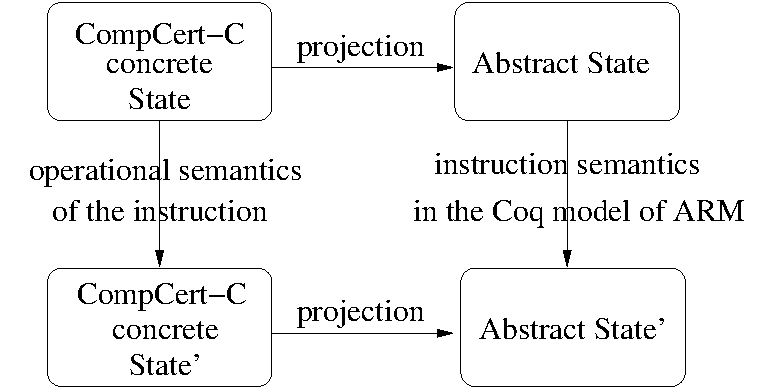
\includegraphics[width=.75\linewidth]{fig/theoremca.pdf}
\caption{More accurate theorem statement for a given ARM instruction}
\label{fig:theoca}
\end{figure}

Recall that our Coq model keeps everything as simple as possible and exactly
corresponds to the ARMv6 reference manual,
whereas the C representation is designed for high simulation speed.
Moreover, additional complexity is introduced because
a suitable memory model is required.

% % JF: useless now
% The projection is dealing with two different value storing systems.
% % JF: irrelevant
% On the right-hand side,
In the \compcert C model, variables are stored in the memory model.
This \compcert C memory model is detailed % "detailed" better than "complex" here
enough to describe the real memory properties,
but it is too complicated to use for computation.
\compcert handles another auxiliary parameter \emph{env},
the local environment.
It maps each variable identifier to its location and its type,
and its value is stored in the associated memory block.
% % JF: don't write this in written style, this is for oral explanations
% It helps us to find what we want in memory.
%
% JF->XM: for what follows I'm unsure to understand what you mean, pls check
% Messy original (your sentences NEVER start at column 0) is below
%\margjf{3}{XM please check}%
The value associated to a C variable or a parameter of a C function
is obtained by applying \texttt{load} to the suitable reference block in memory.
%
However,
this makes sense only after variable are allocated and initialized --
these two operations are performed when a function is called,
building a local environment \texttt{e} and an initialized memory state \texttt{m}.
Similarly, our projection makes sense only at this stage,
i.e., parameters representing the processor state are stored in memory.
Our Coq model of ARMv6 is of course much simpler
and computing the value of a component can be performed directly.

%  This \emph{env} is
% built from allocating function parameters and variables.  Then using
% \texttt{load} from the reference block in memory, we can have the
% value of requiring variable.  The projection is sound if and only if
% the variable allocation and initialization is finished. After these
% two processes, local environment \texttt{e} and an initialized memory
% state \texttt{m} will be constructed. And parameters like processor
% state now exist in memory.  In our own Coq model of ARMv6, we do not
% have such memory model. The variable can be got and computed directly.

% JF: material partly moved above.
% We built projection orientation form \compcert C to our Coq model.
% The two models have different representations of the key variable processor
% state.  Our Coq model keeps everything as simple as possible and exactly
% corresponds to the ARMv6 reference manual. The C model is designed to
% be more complex. Because it considers not only a complete
% representation of ARMv6 architecture but also a high simulation
% speed, optimization on type has been made.

The abstract state of the processor in our Coq model is a record.
It contains two records: one represents the main processor;
the other has the system control co-processor(\texttt{SCC})
and a simple ARMv6 memory altogether.
In the main processor record, the field \texttt{CPSR} (Current Program Status Register)
is defined as a word;
\texttt{SPSR} (Saved Program Status Register)
is a word depending on current processor mode;
\texttt{reg} maps the register to its value as a word;
\texttt{exn} is a list of possible exceptions, which is not in use yet.
\texttt{mode} is a numeration type for all processor modes.
In \texttt{SCC}, there are only two elements,
\texttt{reg} and \texttt{mem}:
\texttt{reg} is the register owned by \texttt{SCC},
which maps the register identical number to its word value;
\texttt{mem} is the ARMv6 memory model, which is a simple mapping from
address to word value.
% XM
% We do not have the MMU (Memory Management Unit) for the moment.
% JF (please check): anyway you had a contradiction with thee next sentence
% which speaks about MMU!
We only have a trivial MMU (Memory Management Unit) for the moment.

\sloppy
%\margjf{4}{I'm confused: the figure says cpsr, not CPSR, etc.}
The ARMv6 Processor data structure in C is given in Figure~\ref{fig:procc}.
It is a \emph{struct}  with thirteen fields,
which in turn contains three \emph{struct}:
\texttt{SLv6\_MMU},
\texttt{SLv6\_StatusRegister} for \texttt{cpsr},
and \texttt{SLv6\_SystemCoproc},
an array of \emph{struct} \texttt{SLv6\_StatusRegister} for \texttt{spsrs},
and six arrays for registers under each processor mode.
The other three are:
an identifier \texttt{id},
which is used when an embedded system has a multi-core architecture;
a pointer \texttt{pc},
which points to the fifteenth of register array under user mode;
and a boolean \texttt{jump} for expressing that the last instruction modifies
the \texttt{pc}, to be cleared after each cycle.
% Oral style
% Let us go back to look at the \emph{struct} \texttt{SLv6\_StatusRegister}.
The \emph{struct} \texttt{SLv6\_StatusRegister}
describes the status register, with bits represented as byte fields,
plus one field to identify the current processor mode.
The datatypes \texttt{CPSR} and \texttt{SPSRS} use this type.
The difference is that not every processor mode has \texttt{SPSRS}.
So an array for \texttt{SPSR} is used under every possible processor mode.
\fussy

% % JF->XM: commented out because not so useful/right/relevant. We can discuss.
%
% To have a complex types can make it much more efficient to reach the
% frequently used data field.  For example, the value of \texttt{CPSR} is a 32
% bits word in our Coq model, but in \compcert C model, it is defined as
% a structure, every significant bit is a field.  In instruction
% operations, it often discusses whether a bit, like \texttt{Nflag} in
% \texttt{CPSR}, is set or not. Then it is easier to get a bit value than
% calculate from a word.  There are more cases like this in C model of
% ARMv6. So the processor data structure is much more complex.  The
% projection has to be defined first for every module that we have in
% processor state of C, and then together they form the whole processor
% state of formal model.

% % JF->XM: Most contents here is trivial or chatting.
% % More useful : give some code of the projection

% \jf{Some code of the projection + comments.
% In particular, comment a little bit on \texttt{load}
% Refer to Fogure~\ref{fig:proj}.
% }

The top definition of the projection is shown below.
Each sub projection refers to the link between
an concrete element and its abstract version,
in red color in Figure~\ref{fig:proj}.

\begin{alltt}
Definition proc_proj (m:Mem.mem) (e:env):Arm6_State.state:=
  Arm6_State.mk_state
    (Arm6_Proc.mk_state
       (cpsr_proj m e)
       (spsr_proj m e)
       (regs_proj m e)
       nil
       (mode_proj m e))
    (Arm6_SCC.mk_state
       (screg_proj m e)
       (mem_proj m e)).
\end{alltt}

For example, the projection for registers owned by the main processor is
called \texttt{regs\_proj},
which takes the C memory state \texttt{m} and the local environment
\texttt{e} as arguments and return \texttt{register -> word}.
The definition is as follow:

\begin{alltt}
Definition regs_proj (m:Mem.mem) (e:env): register -> word :=
  let load_reg id n m e:=
    match find_reg m e id with
      | Some(Vptr b ofs)=>
        load_val (Mem.loadv Mint32 m (Vptr b (add ofs (repr n))))
      | _ =>Int.zero
    end in
    fun r =>
      match r with
        | R k => load_reg user_regs k m e
        | R_svc k _=> load_reg svc_regs k m e
        | R_abt k _=> load_reg abt_regs k m e
        | R_und k _=> load_reg und_regs k m e
        | R_irq k _=> load_reg irq_regs k m e
        | R_fiq k _=> load_reg fiq_regs k m e
      end.
\end{alltt}

Using the name of the register group as index to find the associated
memory block, from which the value is loaded.
Loading from memory state requires also the chunk information of its
type, size and signedness, and the offset.
In this case, the chunk of register is \texttt{Mint32} which means
it is 32-bit integer.
If the corresponding register is not found in memory state,
it returns zero. Initially, the value stored in register is zero.

According to the type of the argument on the right hand side of the
projection, the definitions of projections are quite different.
For example, the projection of a register given above
performs a case analysis on a value of type \texttt{register},
whereas the projection of SPSR depends on the type of exception modes.
We define a specific projection for each type.
Coq is rich enough to allow us to define a general projection
for all types of elements,
using dependent types.
However the gain in clarity of the specification is unclear,
and it would anyway be just a wrapper around specific projections,
so we did not build general protection for parameters.
For improving readability of the statement,
we even chose to define a projection relation for each instance.
For example, the projection relation of register Rn is :

\begin{alltt}
Definition rn_related (m:Mem.mem) (e:env) (rn:regnum):Prop :=
  reg_proj m e n = rn.
\end{alltt}



% To express the projection between the two representations of ARMv6 processor,
% we need two elements:
% the memory state where the variable is stored in the \compcert C model
% and the corresponding variables representation in formal model.
% Here we assume that in the \compcert C side,
% the memory is already allocated completely the variables of
% an instruction. Then the processor state and other parameters must
% exist in the current C memory state without doubt.
% So we can directly use the \coqdocvar{load} function to get the content
% of given block, without considering the memory reading mode, or if the type
% of the variable is volatile.
% The only problem is that the processor state is a quite complex structure in
% C side. The loading operation could not be simple and flat, and always
% contents more than one level loading for a data field.
% We have to first be very careful and with fully understanding of the
% C data structure to be sure that this manually written interactive with
% memory will not be error-prone.
%
% According to the definition in Coq formal model, processor state describes
% the instruction execution status in three conditions,
% \coqdocvar{Ok}, \coqdocvar{Ko}, and \coqdocvar{Todo}.
% Then there are three situations of projection for each corresponding Coq processor state.
% The state of formal model is detailed in Section~\ref{ssec:fsmoa}.
% So we are able to speak whatever happened in C ARMv6 model,
% we can find a corresponding state in the formal model.

\begin{figure}[h]
\hfil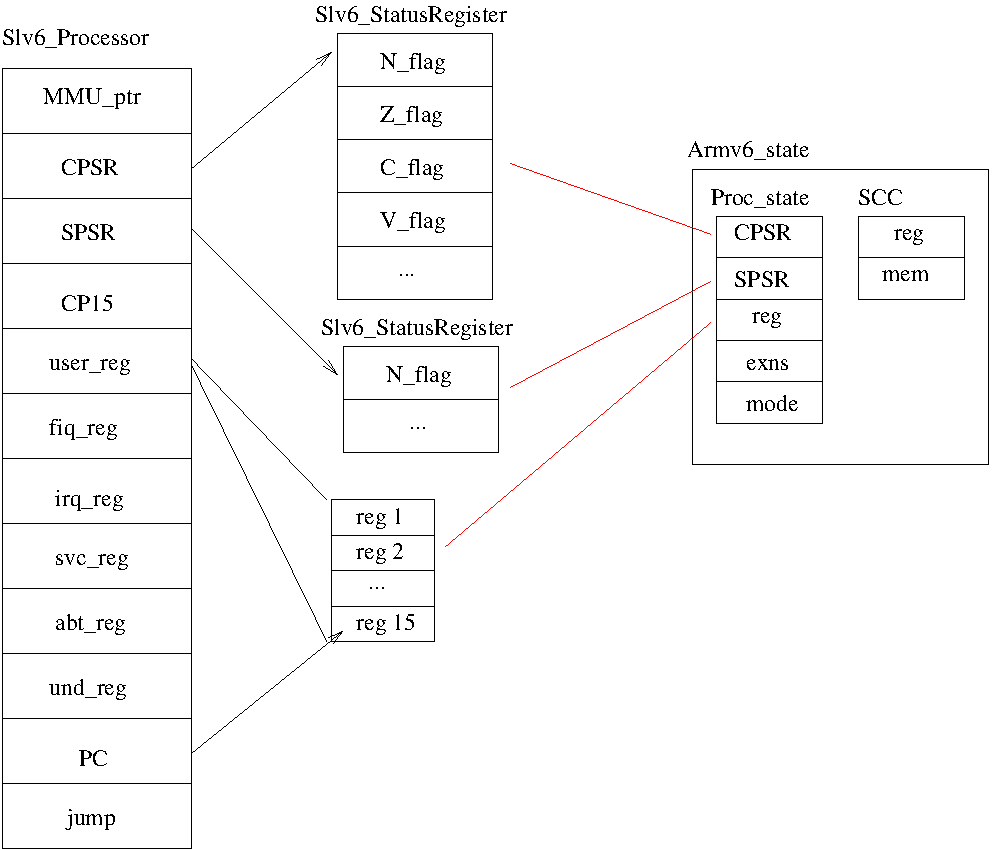
\includegraphics[width=.75\linewidth]{fig/projection.pdf}
\caption{Projection}
\label{fig:proj}
\end{figure}

\sloppy
% % JF -> XM: congratulations, your analysis sounds very good :)
In another project in our group called CCCBIP,
another way is used to express the projection.
The \texttt{eval\_expression} is reused to link the memory state
and the variable value:
$$G,E\vdash \texttt{eval\_expression}~(Ederef(Evalof(Evar x)))~M~\Rightarrow M,~v.$$
The value of $x$ in the formal model is $v$ and the \compcert C expression
$Ederef(Evalof(Evar x))$ is used
to dereference the variable $x$ from the memory contents.
In this case
the memory state remains the same because this evaluation only reads from memory.
This technique can be used there because the type of values are very simple
(integers).
On the contrary, the types in \simsoccert are much more complex:
we have structure pointers inside structures, or arrays of structures
inside structures, etc.
Simply dereferencing with $Ederef$ as in CCCBIP would raise issues in our case.
Manually writing such expression would become error-prone.
Even more, this method results in more inverting tactics during proving,
which makes the proof script harder to follow.
And after inverting, the function \texttt{load\_value\_of\_type}
(or \texttt{deref\_loc}), which loads from memory,
will be added to hypotheses as the premise of evaluating the right value of expression
\texttt{Evalof}.
And it is just the same as the \texttt{load} function with premises
on memory access mode predicate and type volatile judgment.
But these premises would then be redundant with the existing
hypotheses obtained during analyzing the evaluation of the expression
where the corresponding variable is mentioned.

\fussy

\section{Proofs}

\subsection{Proofs for an ARM instruction}
\label{ssec:prfinstr}

%%how many internal memory states


The correctness proof is based on the semantics of the formal model
and the \compcert C representation.
The semantics in the formalization is explained in Section~\ref{ssec:fsmoa}.
\compcert designed a semantics for \compcert C in both small-step and big-step.
The big-step inductive type for evaluating expression is enough for our proof.
The semantics is defined as a relation between an initial expression and an output
expression after evaluation.

% JF -> XM: don't chat.
% The first thing to do is to understand the semantics definition in \compcert.
As mentioned before, the semantics of \compcert C considers two environments.
The global environment \emph{genv} maps
global function identifiers, global variables identifiers to their blocks in memory,
and function pointers to a function definition body.
The local environment \emph{env} maps local variables
of a function to their memory blocks reference.
When the program starts its execution, \emph{genv} is built.
On the other hand, \emph{env} is built when
the associated function starts to allocate its variables.

% \noindent\jf{XM: I'm confused by the original paragraph
% so I propose something different and as short as possible,
% which may be wrong, pls check}.

To state the correctness theorem,
we compare a \compcert C function corresponding to
an ARM instruction with its formal definition in Coq.
% To state the correctness theorem,
% we choose to compare between a \compcert C function of
% instruction operation to its formal definition in Coq, instead of a whole program.
% That is because the execution of program discusses
% a \emph{state} that wraps current function,
% current statement, the continuation together with local environment, and memory state.
% The thing we want to discuss is if the projection still hold after executing one
% instruction.
% The value related to projection is just in memory.
% So the only valuable information is memory state who stores the variables we want
% to compare, and local environment helps us to find their memory address.
% % JF -> XM: distracting
% % And we do not need to discuss if the program terminated.
% So the \emph{state} contains too much information than we require,
% and it will bring difficulties to the
% correctness proof on things we do not need.
% The precise requirement is the memory
% state transition and evaluation of statement; in another word is executing the
% function body of instruction definition.
For such functions, it is enough to focus on the part of the concrete state
which is defined by the local environment.
We then consider a projection from the local environment to the abstract state
defined as follows.

\begin{alltt}
Inductive proc_state_related : Mem.mem -> env -> @result unit -> Prop :=
  | proc_state_related_ok :
      forall m e l b, proc_state_related m e
                        (Ok tt (mk_semstate l b (proc_proj m e)))
  | state_not_ok: forall e m mes, proc_state_related m e (Ko mes)
  | state_todo: forall e m mes, proc_state_related m e (Todo mes).
\end{alltt}

\noindent
The shape of the main theorem of an instruction is then:
\newcommand{\textmem}[1]{\textcolor{blue}{\texttt{#1}}}

\begin{alltt}
Theorem correctness\_instr:
  \(\forall\) e \textmem{m0} \textmem{m1} \textmem{m2} \textmem{mfin} vargs st other\_params out,
  alloc\_variables empty\_env \textmem{m0} (fun\_internal\_B.(fn\_params) ++
                                  fun\_internal\_B.(fn\_vars)) e \textmem{m1} ->
  bind\_parameters e \textmem{m1} fun\_internal\_B.(fn\_params) vargs \textmem{m2} ->
  (forall m ch b ofs, Mem.valid\_access m ch b ofs Readable) ->
  proc\_state\_related \textmem{m2} e (Ok tt (mk\_semstate nil true st)) ->
  other\_params\_related \textmem{m2} e other\_params ->
  exec\_stmt (Genv.globalenv prog\_bl) e \textmem{m2} fun\_internal\_B.(fn\_body)
                                       Events.E0 \textmem{mfin} out ->
  proc\_state\_related \textmem{mfin} e (S.instr\_step other_params
                              (mk\_semstate nil true st)).
\end{alltt}

\noindent
Let us explain it in more detail.
\begin{itemize}
\item
  In order to get the projection of the pair of original states, we need
  the following data: the initial memory state, the local
  environment, and the formal initial processor state.
  Recall that the projection is meaningful only after the C memory state
  is well prepared for evaluating the current function body.
  In the abstract Coq model, we directly use the processor
  state \texttt{st}.
  But on the C side, the memory state must provide the
  contents of every parameter, especially the processor state.
  We also need to observe the modification of certain blocks of memory
  corresponding to local variables.
%  a complete local environment -- a map from identifiers to address.
  Therefore, on  \compcert C side, a memory state and a
  local environment is prepared using following two steps.
\begin{itemize}
\item Allocating function variables: from an empty local environment,
  all function parameters and local variables ara allocated into
  the memory state \textmem{m0}, yielding a new memory state
  \textmem{m1} and the local environment \texttt{e}.
\item
Initializing function parameters: using \texttt{bind\_parameters} to initialize
parameters with a list of argument values \texttt{vargs}, a new memory state
\textmem{m2} is created.
\end{itemize}
\item
Now we have all elements for the projection to make sense are ready.
As the most important parameter of instruction operation,
the projection is first applied to \textmem{m2},
and we expect to get the initial abstract processor state \texttt{st}.
\item
The projection is also used on the other instruction parameters.
\item
Then the body of the function is executed.
On the \compcert C side, this is performed using a call to \texttt{exec\_stmt},
yeilding a new memory state \textmem{mfin}.
On the abstract side, the new processor state is obtained using \texttt{instr\_step}.
\item
Finally, we claim that the projection from the concrete state \textmem{mfin}
should provide the latter abstract state.
Note that all projections are performed using the same local
environment \texttt{e}.
\end{itemize}

The proof is performed in a top-down manner. It follows the definition of the
instruction, analyzing the expression step by step.
% % JF->XM as far as I understand it seems not important.
% And one proof block focuses on single expression unit.
The function body is split into statements and then into expressions.

% % JF
When evaluating an expression, we search for two kinds of information.
One is how the memory state changes on \compcert C side; the other is
whether the results on the abstract and the concrete model are related
by the projection.
To this effect, we use six kind of lemmas.
% % XM
% To complete the proof for main theorem, lemmas are required. Lemmas
% that can be categorized in four kinds shown below.  When evaluating an
% expression, there are two things we want to know.
% One is how the memory state changes on \compcert C side;
% the other is what is the outcome result by evaluating an expression
% when two sides are equivalent.

% what is the outcome result by evaluating an expression when two sides are equivalent.

\begin{enumerate}
\item
\textit{Evaluating a \compcert expression with no modification on the memory state.}\\
Such a lemma only discusses the expression evaluation on \compcert C side, involving
with the C memory state changing issue.
Saying a memory state is not modified has two aspects:
one is that the memory contents are not modified; the other is that the memory access
permission is not changed.
For example,
evaluating the binary expression $Sbit~==~1$ returns
% a new memory state, which is equivalent to input memory state.
an unchanged memory state.
\begin{align*}
&\textrm{if}~~ G,E~\vdash \texttt{eval\_binop}_c~(Sbit~==~1),\:M~\xLongrightarrow{\varepsilon}~vres,\:M'\\
&\textrm{then}~~ M=M'.
\end{align*}
% \begin{itemize}
% \item
%   if $G,E~\vdash \texttt{eval\_binop}_c~(Sbit~==~1),~M\xLongrightarrow{\epsilon}vres,~M'$,
% \item
% then $M~=~M'$.
% \end{itemize}

In Coq syntax, the relation in premise is expressed with \texttt{eval\_binop},
a companion predicate of \texttt{exec\_stmt} above,
devoted to binary operations.
In this lemma and the following,
$E$ is the local environment, $G$ is the global environment
and $M$ is the memory state;
$\varepsilon$ is the empty event (\texttt{Events.E0} in Coq syntax);
usually $t$ is used to represent a series of system events; $vres$ is the result.
%$\texttt{eval\_binop}_c$ is the semantics of \compcert C for evaluating binary operation.

Here, $vres$ is not important.
% % JF->XM: useless (redundant)
% We want to prove that the memory state does not change and,
% if nothing change on the abstract side as well,
% the projection will hold again after performing the evaluation.
The evaluation is performed under environments $G$ and $E$.
Before evaluation, we are in memory state $M$.
With no event occurring, we get the next memory state $M'$.
The proof is easy. According to the definition of \texttt{eval\_binop},
an internal memory state will be introduced.\\
\begin{center}
$\dfrac
{G,E~\vdash a_1,M\Rightarrow M'~~~G,E~\vdash a_2,M'\Rightarrow M''
}
{G,E~\vdash (a_1~binop~a_2),M\Rightarrow~M''}$
\end{center}
% \begin{center}
% $G,E~\vdash a_1,M\Rightarrow M'~~~G,E~\vdash a_2,M'\Rightarrow M''$\\
% \line(1,0){220}\\
% $G,E~\vdash (a_1~binop~a_2),M\Rightarrow~M''$
% \end{center}
Now, in our example, expression $a_1$ is the value of $Sbit$
and $a_2$ is the constant value $1$.
By inverting the hypothesis of type \texttt{eval\_binop},
we obtain several new hypotheses,
including on the evaluation of the two subexpressions
and the introduction of an intermediate memory state $M''$.
Evaluating them has no change on the C memory state.
Then we have $M = M'' = M'$.

In more detail, from the \compcert C semantics definition, we know that,
evaluation of an expression will change the memory state if
the evaluation contains uses of \texttt{store\_value\_of\_type}
(in \compcert versions before 1.11),
which stores the value in memory at a given block reference
and memory chunk. %  of reference type. % JF complicated...
In \compcert-1.11,
the basic store function on memory is represented by
an inductive type \texttt{assign\_loc}
instead of \texttt{store\_value\_of\_type}.
Since \compcert version 1.11 introduces volatile memory access,
we have to determine whether the object type is volatile before storage,
and also type size in addition of the access mode.

\item
\textit{Result of the evaluation of an expression with no modification on the memory.}\\
Continuing the example above, we now discuss the result of evaluating
the binary operation $Sbit~==~1$ both in the abstract and the concrete model.
At the end of evaluation, a boolean value $true$ or $false$ should be returned.
% Now we consider both sides of the projection.
% %JF -> XM "projective variable" does not exist
% First, we need to find the pair of projective variable $Sbit$
in \compcert C model and Coq model,
using the projection definition we introduced in~\ref{sec:proj}.
% \jf{I think that arguments are missing for \texttt{parameter\_related}:
% I intuitively expect a memory, an environment,
% an identifier for the name of the parameter, say \texttt{sbit},
% and an expected value, say $Sbit$. Not sure of the font to use.
% Make a choice and be consistent with the use of fonts,
% it is important for understanding,
% and showing that you understand what you write.
% Give the definition of \texttt{parameter\_related}.
% It is probably better to do that earlier, with \texttt{proc\_related}
% in the previous subsection.}
%
\begin{align*}
&\textrm{if} ~ \texttt{Sbit\_related}~M~\texttt{Sbit},\\
&\textrm{and} ~ G,E~\vdash \texttt{eval\_rvalue\_binop}_c~(Sbit~==~1),M\Rightarrow~v,\\
&\textrm{then} ~ v=(Sbit~==~1)_{coq}
\end{align*}
%
Intuitively,
if the projection corresponding to the parameter \texttt{sbit} in the C program
yields the right information from the abstract state,
then the evaluation will return the same value both
in the abstract and in the concrete model.
Here, the expression is a so-called ``simple expression''
that always terminates in a deterministic way, and preserves the memory state.

To evaluate the value of simple expressions,
\compcert provides two other big-step relations \texttt{eval\_simple\_rvalue} and
\texttt{eval\_simple\_lvalue} for evaluating respectively their left and right values.
The rules have the following shape:
\[
\dfrac{
\begin{array}{l}
G,E~\vdash a_1,M\Rightarrow v_1 \quad G,E~\vdash a_2,M\Rightarrow v_2\\
\texttt{sem\_binary\_operation}(op,v_1,v_2,M)~=~v
\end{array}}
{G,E~\vdash (a_1~op~a_2),M\Rightarrow v}
\]
In order to evaluate the binary expression $a_1~op~a_2$,
the sub-expressions $a_1$ and $a_2$ are first evaluated,
and their respective results $v_1$ and $v_2$ are used
to compute the final result $v$.

\item
{\it Memory state changed by storage operation.}\\
As mentioned before, evaluating some expressions such as \texttt{eval\_assign}
can modify the memory state.
Then we need lemmas stating that corresponding variables in the abstract
and in the concrete model will evolve consistently.
For example, this is stated as follows for an assignment on register $Rn$.
Here we use the projection relation \texttt{register\_related}.

%\jf{Put the definition of \texttt{register\_related} in the previous section.}
% \jf{But again I don't understand: there should be an argument for the name of the register,
% say \texttt{n} or  \texttt{Rn}
% and another for the value contained in the abstract model, say $rn$;
% moreover $M$ is rightly changed in $M'$,
% but I would expect $v$ instead of $rn$ in the conclusion.}
\begin{align*}
&\textrm{if} ~~ \texttt{rn\_related}~M~rn\\
&\textrm{and}~~  G,E~\vdash \texttt{eval\_assign}_c~(rn:=rx),M~\Rightarrow~ M',v\\
&\textrm{then} ~~ \texttt{rn\_related}~M'~rn
\end{align*}

\item
\textit{Evaluating expressions with modification on the memory.}\\
This is similar to the previous case.
% This is one of the cases that the memory state is modified, some of the memory blocks
% represent fields of processor state is modified. And a new projection will be hold.

\item
\textit{Internal function call.}\\
% To deal with the internal function calls, our translated code is not enough.
Internal functions are described in an informal manner in the ARMv6 reference manual.
No pseudo-code is available for them,
which means that the corresponding library functions,
both in the abstract Coq model and in \simlight,
are written by hand.
In order to get a suitable \compcert C AST to reason about,
we use the parser provided in \compcert.
% The translated code is from pseudo-code AST to \compcert C AST and prints them into
% Coq representation, which only contains the definition of instruction operation.
% Then we have no definition on the library function. We have to either
% define them manually by reading the reference or reuse part of the \compcert
% compiler, the parser from normal C
% code to \compcert C AST, in order to obtain the function bodies from the
% hand-written C definition for library functions in \simlight.
% Then add them to the translated code.
When combining the simulation code of an instruction with the
code of library functions,
we need to take care of the memory allocation problem.
In \compcert C representation, identifiers are unique positive numbers
which indicate the memory block where corresponding variables are allocated.
Currently, the extra identifiers introduced by library functions are
added manually and assigned with fresh block numbers.
\label{page:libfunast}
% \jf{Something missing here to explain what is the problem with these numbers,
% and which processes can be automated in future work.}
% \xm{Both processes can be represented automatically.
% This can be a future work to be completed. }
%
\begin{align*}
&\textrm{if} ~~  \texttt{proc\_state\_related}~M~st\\
&\textrm{and} ~~ G,E~\vdash \texttt{eval\_funcall}_c~(copy\_StatusRegister)_c,M\Rightarrow~v,~M'\\
&\textrm{and} ~~ st'~=~(copy\_StatusRegister)_{coq}~st \\
&\textrm{then} ~~\texttt{proc\_state\_related}~M'~st'.
\end{align*}
% \begin{itemize}
% \item
% if $\texttt{proc\_state\_related}~M~st$,
% \item
%   and $G,E~\vdash \texttt{eval\_funcall}_c~(copy\_StatusRegister)_c,M\Rightarrow~v,~M'$,\\
%   and $st'~=~(copy\_StatusRegister)_{coq}~st$
% \item
% then $\texttt{proc\_state\_related}~M'~st'$.
% \end{itemize}

After an internal function is called, a new stack of blocks is
allocated in memory.
After the evaluation of the function is performed, these blocks will be freed.
Unfortunately, this cannot bring the memory back to the previous state:
the memory contents may stay the same,
but the \texttt{nextblock} pointer will skip these just freed blocks and point
to the followed block.
% \jf{What do you intend to say in the next sentence? That equal memories
% is too restrictive I guess?
% So what? Do you have a suitable ``equivalence'' predicate on memories?
% Seems that the answer is no.
% I guess that you just say that some observations on memory will
% provide the expected result.
% Is it right? And is it enough for performing the next proof steps,
% which may require resoning on many projections?}
% \xm{To state that two memory states are the same means that
% their memory contents, the memory access permission, the next block, and so
% on, should all be the same.}
For lemmas on evaluation of internal functions,
we can observe the returned result on variables and compare it
with the corresponding evaluation in the formal specification.
For example,
the lemma above is about the processor state after evaluating an internal
function call \texttt{copy\_StatusRegister} which reads the value of
CPSR and then assigns it to SPSR.
% It always follows the condition. JF->XM: which one? Seems redundant anyway.
The evaluation of \texttt{copy\_StatusRegister} should be protected by
a check on the current processor mode.
If it is neither system mode nor user mode,
the function \texttt{copy\_StatusRegister} can be called.
Otherwise, \simlight % the simulation system; JF->XM: correct? Yes.
will return ``unpredictable'' with an empty message.

% \texttt{copy\_StatusRegister} is defined differently in two side.
% Every time when we want to perform copying from CPSR to SPSR, we have to
% first check if current mode has SPSR. That means function
% \texttt{copy\_StatusRegister} always follows the condition judging which is
% the current processor mode, and if current mode does not have SPSR it will return
% an empty message.

Then we have to reason on the newly returned states,
which should still be related by the projection.
This step is easy to prove by calculation, simplifying on
two representations of the processor state.

% JF HERE
\item
\textit{External function call.}\\
% \jf{Question to XM:
% from what you say something is unclear to me:
% is it feasible to perform proofs, or just impossible?
% When you say that ``only few built-in external
% functions have their certain semantics'' (I'll rephrase)
% does it mean that \compcert provides an axiomatic
% description of these functions?
% And that the implementation in assembly code is proven
% correct wrt. these axioms?
% At the moment I write something else.
% Note that I'm NOT sure at all, I just GUESS.
% It seems better to distinguish external functions and external function calls.
% Please check.}\\
% Currently, we do not consider external function calls in C representation.
% Because \compcert C has not
% yet supported self defined external function calls, only few built-in external
% functions have their certain semantics. If we have an external function call in
% C code, the translated \compcert C representation will have an empty body for
% external function, containing only the input argument type and the returned value
% type.
% We can only reason about:
% External functions are not part of the \compcert C language.
% They only can be described in an axiomatic way.
The \compcert C AST of an external function call contains
the types of input arguments and of the returned value,
and an empty body.
\compcert provides the expected properties of a few
built-in external functions such as \texttt{printf},
\texttt{malloc} and \texttt{free}.
We proceed similarly for the external functions of \simlight.

% % JF: moved here this paragraph which was after the list
% In general, we expect the result returned by evaluation of external function.
% But there is no semantics provided on the self defined external function body.
% In \simlight, some functions are defined as external ones.
% This is for modularizing the simulator. %  to make it clean %% Of course!!
% Even it is a simplified version of the large \simsoc simulator,
% it is still a quite complex system.
% So the problem left for us is to either change all the external
% functions into internal or give assumptions every time we meet
% external.
%
% % JF Rewriting this paragraph, removing redundancies
% \jf{Email sent, check/rewrite according to answers.}
In \simlight, some functions are defined as external ones
-- something which is needed even is this simplified version of \simsoc.
They could be changed into internal functions in the future
but in the current version, they are left external.

The general expected properties of an external call are as follows.
\begin{itemize}
\item
  The call returns an result, which has to be related to the abstract.
\item
  The number of arguments must agree with the signature.
\item
  After the call, no memory blocks are invalidated.
\item
  The call does not increase the max access permission of any
  valid block.
\item
  The memory state can be modified only when the
  access permission of the call is the maximal.
\end{itemize}

% Currently, we can only give \texttt{Axiom} on external function about the execution
% result.
% According to the given property, evaluation of an external function will not change
% the original memory contents.
% Then it is better to return the execution result in a variable.
% The common \texttt{Axiom} looks like:
For \simlight, the result of an external call is written in a variable
such as \texttt{vres} in the next example.
A typical axiom for stating that the external function \texttt{ef\_c}
returns a result specified by the Coq expression \texttt{ef\_coq} is:
\begin{alltt}
Axiom res_extcall :
  forall m ef_{c} targs tres vargs t m' vres,
    eval_funcall m (External ef_{c} targs tres) vargs t m' vres ->
    vres = ef_{coq}.
\end{alltt}
%The result of executing function $ef$ on both sides will be the same.
\end{enumerate}

\subsection{Proof design}
% % JF -> XM: the following is about prof technique and currently obscure
% % therefore probably less important than the other on structuring into lemmas.
% % I moved it

%% JF->XM: this is well-known
% During the proof process, some proof strategies are frequently used.
% Repeating every time the same proving steps is repetitive and time consuming work.
% It is better to have lemmas on them.
% Or even we can define our own tactics to have these steps done in one move.
As usual, repetitive steps in proofs are dealt with using auxiliary lemmas and
dedicated tactic definitions.
In our case,
% most of this work is done for \compcert C side.
most of them are related to the semantics of \compcert C.
Indeed, since the abstract Coq model is defined in a functional style,
many proof steps are just reductions using, e.g., \texttt{simpl} or \texttt{unfold}.
% One reason is that semantics is defined in functional way in the formal model.
% The execution result can be carried out by simplifying or unfolding
% the functional definition.
In contrast, the execution of a C program is provided by a inductively defined
relations, the operational semantics.
Decomposing this execution step by step amounts to perform so-called \emph{inversions}
on hypotheses relating concrete memory states according to the operational semantics.
In practice, a large amount (several dozens) of inversions are performed,
bringing serious issues on space-time consumption and maintenability.
We studied a general solution to this problem, to
% But in \compcert side, to find a execution result we have to follow step by
% step the premises which are defined in the semantics inductive types.
% This means that there are really a lot of inversions on hypotheses.
% The issue on inversion brought us much inconvenience in our proof scripts,
% like scripts size, time consumption, naming issue.
% The way to improve the proof strategy will
be introduced in Chapter \ref{cpt:inv}.

More specifically,
back to the design of proofs,
here are the main issues and how they are dealt with.

%\begin{itemize}
\paragraph{Getting a usable local environment.}
% % JF: Seems to be useless
% The importance of parameter local environment is mentioned above.
%
We often need to consider whether a variable exists in C memory or not,
and to get the corresponding location in memory.
To this effect, the concrete contents of the local environment \texttt{e} is required.
To achieve this,
inversions are systematically performed on \texttt{alloc\_variables} hypotheses.
Then \texttt{e} becomes a \emph{closed} (and reduced)
mapping indexed by variable identifiers
(before, \texttt{e} is just a variable having the type of a mapping).
%
% % JF-> XM : your proving strategy is not defined (at least at this point)
% Through the proving strategy, we often consider whether a
% variable exist in C memory or not.  It is necessary to have a concrete
% mapping \textbf{e}. Then it is possible to look for variable locations
% in memory. To achieve this, the operation \texttt{alloc\_variables}
% has to be inverted for each argument of a function.
%
\paragraph{Finding a variable location in memory from its  identifier.}
This is simply solved by applying the \texttt{get} operation
provided by \compcert on the local environment~\texttt{e}.
This computation can actually be performed when~\texttt{e} is closed.
% Using the concrete local environment, it is possible to judge whether
% a variable reference has a corresponding location in memory or not.
%  It is simply using a get in tree structure with index.

\paragraph{Finding a function location in memory.}
Two kinds of functions exist in C.
Internal functions are in the local environment \texttt{e},
whereas external functions are in the global environment \texttt{g}.
When a function reference is met,
a \texttt{get} operation is invoked on \texttt{e},
then on \texttt{g} in case of failure.
% In C, there are two kinds of functions: internal functions and external
% functions.  When we meet a function reference, in order to know which
% kind it is, we have to look up into the local environment first. If it
% exists in the local environment, it is internal.  If not, we search it in
% the global environment. If it exists in global environment, it is
% external. Whether searching in local or global environment, it is to
% \texttt{get} from a special tree with a reference.

\paragraph{Evaluating memory states.}
\compcert C semantics operates on memory states.
% % XM
% To observe
% JF
Observing
them is essential, in particular to compare the concrete state with
the expected abstract state.
The memory state stays unchanged,
except when a \texttt{store} occurs during evaluation.
In the inductive relation \texttt{eval\_expr},
this only happens for an assignment (\texttt{eval\_assign}),
an assignment with arithmetic operation (\texttt{eval\_assignop})
or a post-increment operation (\texttt{eval\_postincr}).
% JF -> XM: the following is wrong (it is correct only for base cases)
% All the other expressions will not change the memory state.
Whatever the expression, it has to be analyzed and recursively decomposed
in order to get closed (then usable) memory states.
Again, this is performed using inversions on \texttt{eval\_expr} hypotheses.
The inductive type \texttt{eval\_expr} is big and expressions in
\simlight are complex,
raising serious issues with the Coq standard tactic \texttt{inversion}.
We then decided to write our own inversion tactic.
We go back to this in Section~\ref{sec:ninv}.

\paragraph{Analysing values in a memory block.}
The \compcert memory model includes four kinds of operations:
\texttt{load}, \texttt{store}, \texttt{alloc}, and \texttt{free}.
They operate on a memory chunk at a given address.
For these four operations, several properties are provided.
We use them to determine
which block or memory chunk is affected by one of these operations,
and which part of the memory is left unchanged.

%\end{itemize}

\subsection{Proofs for shared library functions}
\label{ssec:cf}

Every ARMv6 instruction contains one or more calls to
internal or external functions. For the moment, the external functions
are not taken into account, for a reason explained in ~\ref{ssec:ccc}.
As mentioned in Section~\ref{sec:arm_ccc},
% % JF: usure of the syntax and anyways, complicates the reading
% % By the way I don't like "instruction operation", looks improper English
% except the instruction operation body,
functions called in an instruction need to be added manually.
Most of these functions are used in different instructions.
% But the proposition we ask from them is mainly the same.
% % JF: remove or simplify the following which is obvious
% Adding them one by one into every instruction and
% having similar proofs everywhere is a rigid work.
% It is better to have their function body declared in a common file and have their
% lemmas shared by all related instructions.
As the properties expected from them are always the same,
we want to state and proof corresponding lemmas once for all.
%
% % JF-> XM: big issue here
% \jf{I'm not sure that you are right: as far as I understand,
% proofs are performed on different standalone programs:
% an independant program for each isntruction.
% As we have different programs, the fact that identifiers cannot
% be repeated is irrelevant, since it is relevant only
% inside a given program.
% Hoowever, I think that we have no control on the identifiers
% representing variable or function names.
% And this is enough to make function be represented by
% different identifiers in different programs,
% hence the issue and the solution with Coq modules.}

One issue from the \compcert compiler is that
% every identifier is a positive number which also
% indicates the location in memory.
% And identifiers cannot be repeated.
identifiers (positive numbers indicating a location in memory)
cannot be repeated:%\margjf{2}{To be changed if previous comment in red is correct}:
these memory locations are settled once a program is evaluated,
and the global environment and local environment will be
filled with allocation information.
% To add a function into a programs,
% we have to re-arrange the memory allocation by giving new blocks to
% the new introduced variables and functions.
The insertion of functions in a program is performed by the
assignment of new blocks to the corresponding identifiers.
The issue is that the same function in different program
will be represented by different identifiers.
We solve this issue using Coq \emph{sections}.
A section is defined for each function
with its associated lemmas.
Its variables are defined abstractly by just giving their types.
% When adopting library function module to a program,
% the assumed identifiers will be assigned to real values.
Integrating such a function into the \compcert code of an instruction
consists in importing the file containing the corresponding section,
instantiating additionally assumed variables with appropriate values,
then performing memory allocation.
% % JF: an adding function is a function for performing addition !!!
% This adding function needs to be done before allocating memory.

% % JF -> XM ??? A library function IS an internal function, no?
% How to perform proving on library function is like the proof for internal
% function, which is explained in Subsection~\ref{ssec:prfinstr}.
Proofs on library functions are performed in the same way as for instructions,
see Subsection~\ref{ssec:prfinstr}.

% In every ARMv6 instruction, operation contains calls to internal or
% external functions. For the moment the external functions are not take
% into count, the reason is explained in ~\ref{sec:ccc}.  We mention in
% previous section \ref{sec:arm_ccc}, except the instruction operation
% body, the other functions call in one instruction need to be added
% manually.  Most of these functions are used in different instructions.
% But the proposition we ask from them is mainly the same.  Adding them
% one by one into every instruction and having similar proofs everywhere
% is a rigid work.  It is better to have their function body declared in
% a common file and have their lemmas shared by all related
% instructions.  In practice, lemmas we stated for each internal
% function are about, whether it have side-effect, if so, the outputs
% should be the same in formal model and \compcert C model. Or some of
% the variable we want to reason about is not changed by such internal
% function.  And the proposition here depends on an abstract memory
% model.  We have to assume there is a block in a memory state refers to a
% definition of an internal function.  Then apply to each instruction,
% these block value will be instantiated according to the current memory model
% build by programs.

\subsection{Proofs on tricky operations on words}
%Except the lemmas on internal functions, there are other library functions about
%comparing the same function defined in different ways,
We also have lemmas for checking that different ways of computing
a function actually provide the same result.
An example is the function for getting the bit at a given position
in a word represented by a binary integer.
The equality to be proved is, after simplification:
\begin{alltt}
\hfil and (shru \(x\) (repr (Z\_of\_nat \(n\)))) (repr 1) = \(x\)\:[\(n\)].
\end{alltt}
It means that the definition of \texttt{get\_bit} used in \simlight
can be (efficiently) computed by a combination of binary operations
\texttt{and} and \texttt{shru} (logical shift right)
on the integer $x$ and the bit number $n$.
On the right hand side,
the formal specification uses a bit mask on the object integer $x$
to get the $n^{\rm th}$ bit.
The comparison is quite complicated due to the range of the result in type integer.
We have to take a restriction into account,
saying that $n$ should be greater than $0$ and less than the word size,
and to add specific lemmas on other arithmetic definitions.

\section{Tactics}
\label{sec:tactic}

Coq provides the Ltac language to allow the user to define her/his own tactics.
% % JF useless
% Like the built-in tactics, we can define our own tactics to apply to goals during Coq proofs.
LTac expressions can be used in the proof script of a given theorem, or in
% This process can be defined during proof or pre-defined as
a top-level Ltac definition.
The most useful
% semantics % JF->XM: Nothing to do with semantics
construct
of Ltac is the pattern matching on a proof goal,
which analyzes the current goal and binds names to useful informations.
This is used for our inversion \hcinv described in Section~\ref{sec:ninv}.
We also defined tactics dedicated to our specific needs,
% helping us to make the proofs easier and systematic.
representing systematic reasoning schemes on the \compcert C semantics.
Most of them deal with the C memory model and with operational semantics rules.
% we have many proof strategy repetitive.
% The most work we are dealing with through all the proof scripts
% is the C memory model and the operational expressions semantics.
% \begin{itemize}
% \item
\subsection{Load/store operations}
% The properties we have to discuss very frequently is
Many reasoning steps are about
the effect of a load/store operation on memory.
% The load/store operations are always bounded
% by the low/high bound of the memory blocks.
Such operations are always constrained by low and high bounds of the memory blocks.
In order to know
whether the memory block we focus on remains the same
or has been changed to a new contents,
we have to determine the range of blocks
% % JF I don't understand. You may mean what I write below
% operated on C memory model
targetted by operations on memory.
%
% % JF I don't understand. Is it related to the previous sentence? If yes how?
% % JF I assume that not (hence "also")
% % JF I don't understand. You may mean what I write below
% We need to reason about the relation of the blocks:
% the ones to load/store; and the ones we want to guard, %JF: what is "guard"? protect?
% whether the two groups of blocks are not overlapped.
We also need to check that a given block do not overlap with other blocks.
%
The position of every variable and function is given during allocation.
In order to find the value of blocks,
we then have to analyze the appropriate allocation hypothesis,
providing information on how the environment is initialized.
This is performed using a series of inversions
because the allocation operation is inductively defined.
The number of inversion steps is equal to the number of variables in the function.
This yields the same number of new hypotheses
indicating the position where each variable is allocated.
The definition of the initialization of a function
ensures that the blocks allocated are pairwise different from each other,
and that the pointer to the next block % of current memory state % JF: obvious
always points to a block which has a greater position number.
% So the problem to be proved is a transmission of
% ``less than'' comparison between the blocks.
After a number of reasoning steps on the ``less than'' relation
between block position numbers,
we apply a suitable lemma provided by \compcert,
\texttt{load\_store\_other} or \texttt{load\_store\_same},
to determine whether the memory state changes after a load/store operation.

%\item
\subsection{Outcome of a statement}

The execution of a statement produces an ``outcome'',
indicating how the execution terminates:
either normally or prematurely through the execution of a
\texttt{[break]}, \texttt{[continue]} \texttt{[return]} statement.
\texttt{Sdo} is a very common statement in \compcert C programs.
It can be used as a wrapper of a single statement.
Executing a \texttt{Sdo} statement always returns \texttt{Normal}
whatever the contents is.
And similarly for statement \texttt{Sskip}:
it is the same as a \texttt{Sdo} with no contents.
% To save time and space for this repetitive work,
In order to manage such situations,
we provide a tactic based on the inversion of % the inductive definition of
the semantics of statements.

%\item
\subsection{Function calls}
% % JF->XM: you should sometimes make a more important effort in
% % - writing things in a right order. Please compare with your previous version.
% % - explaining your intention: what is the purpose of this tactic?

% The last tactics is used in the proof scripts which
% contains the calls to function.
We also have a tactic dedicated to function calls.
It is used in all instructions,
since every instruction has one or more internal function calls.
This tactic aims at finding the block containing the body of the called function.
Indeed, the local environment does not contain functions but only their name.

To find the function, we have to go through the global environment.
The global environment is also defined using the \texttt{PTree} data structure,
which maps a reference to the corresponding place in memory,
or a function pointer to a function definition,
or a variable pointer to the associated contents.
% % JF->XM: I don't understand and it seems to be irrelevant anyway. Right?
% It also restricts the block distributed
% for the next variable or function and their range.

By analyzing the hypothesis for evaluating the function identifier we aim at,
we get a hypothesis $G~\vdash \texttt{find\_symbol}~id~=~\lfloor b \rfloor$,
saying that the global environment $G$ contains a block $b$ for the symbol $id$.
Next, we invert the appropriate \texttt{eval\_funcall} hypothesis:
according to rule~\eqref{eq:funcall} recalled in Subsection~\ref{ssec:ccc},
we get an hypothesis $G~\vdash \texttt{find\_funct\_ptr}~b ~=~\lfloor f \rfloor$,
saying that in the same global environment $G$, using the block $b$,
then we are able to find the function pointer.
Then we use the \texttt{set} and \texttt{get} operations
to explore the global environment, until we find the matching block.
These proof steps are automatically performed in LTac
using pattern matching on goals.


%\end{itemize}



\section{Dealing with version changes of \compcert}

During the development of our correctness proofs,
three versions of \compcert were released,
bringing new features and better performances.
%
The change of version from \compcert-1.8.1 to \compcert-1.9 did not
cause much trouble on \simsoccert.
We discuss here the impact of the next two releases on our project.

\subsection{Changes from \compcert-1.9 to 1.10}

An important fact on version 1.9 is that
it turned the \compcert C reduction semantics into a reference interpreter.
% And bugs have been fixed in the semantics of \compcert C.
% % JF: complicated, so I don't spend time on it unless it is relevant
% Function that calls through function pointer now have a certain semantics to match
% and the conditional expression when the two branches with different types will
% cast them to their common type.
%
Handling of annotation statements has been improved to separate where has
one integer argument and where has arbitrarily many arguments.
And efforts have been done for handling external function
and compiler built-ins.
The built-in external function for memory operation ``copy'' is
now fully specified as well as other changes which we do not care.
We only care about the semantics and part of the low level definitions.
So, \simsoccert only needs to be changed for some small point as the
semantic cast is no longer a inductive type but a pattern-matching function.
The way to apply such cast definition needs to follow the version.
At that time, we have not begun the correctness proof involving the external
functions.
Then the changes due to this part can be ignored.
But the version change of \compcert-1.9 to \compcert-1.10 brought backward
incompatibility to \simsoccert.
Not only because many things have been changed in the newer version 1.10,
but also our \simsoccert project becomes richer
and more stuff depends on \compcert,
especially in the correctness proof scripts.

Next, we introduce the main changes between the two versions and
explain the impact to our project.

\subsubsection{Volatile types}
\compcert C now natively supports volatile types.
Its semantics fully specifies the meaning of accesses to volatile memory,
and the translation of volatile accesses to built-in function invocations
is proved correct.

In order to prepare future evolutions of \compcert,
most constructors of the Coq type \texttt{type} for \compcert C types expect
a record called \texttt{attr} (for attributes),
which is introduced in \compcert-1.10.
Volatility of memory is specified by
a Boolean field in this record.
% The attribute currently only has one field representing
% the volatile memory accesses by a boolean value.
Our generator had to be then changed to take this field into account.
Since the introduction of volatile memory access,
the way to compute the value of a given data is changed.


Introducing the volatile type also changed the
definition of the projection from the concrete to the abstract
representation of the ARMv6 processor,
because of the use of the \texttt{load} operation in this projection.
% The projection obtain the C side value by loading from memory blocks.

% % JF: I guess something, see below

% % JF: repeated below in a better way
% This loading definition is changed from functional to relational now.
\simlight currently includes no volatile variable.
Then we can directly use the normal load
without considering the volatile attribute.
But our correctness proofs are modified,
because the semantics of load/store is no longer given by a functional definition
but by an inductive type,
which is used to express additional concerns about the
volatility of load/store.
The main impact is on proofs related to assignment expressions.

% \xm{%
% Other than computing the access mode (to get the size of a memory chunk we
% want load/store) by its type, we also have to consider the attribute
% of volatile memory access of this type.
% Then to decide it is a normal load/store or a volatile load/store.
% When it is volatile load/store we need to browse in the global environment:
% if the block is marked volatile in global information and if the event value
% can match the type of the block content.
% }

% have to be modified in order to adopt this new type.
% \item
%   Now \compcert C supports the assignment between composite types
%   (structs or unions).  The value can be cast from one argument of
%   type struct/union to another is their types have the same
%   struct/union identifier and the same field list.
\subsubsection{Booleans}
From this version, \compcert C provides Booleans.
% size is specified, distinguished from the other bit size: 8, 16, or 32.
This could be used in \simsoc,
where Boolean values are represented as unsigned 8-bit ints.
However C Booleans are currently not considered.

% The generation ARM instructions in \compcert C can have Bool type directly
% instead of unsigned 8-bit int.

% - Support for \_Alignof(ty) operator from ISO C 2011\\
% and \_\_alignof\_\_(ty), \_\_alignof\_\_(expr) from GCC.\\
% \item
% Performance improvements:\\
% - Improvements in instruction selection, especially for integer casts
% and their combinations with bitwise operations.\\
% - Shorter, more efficient code generated for accessing volatile global
% variables.\\
% - Better code generated for the \&\& and || operators.\\
% - More aggressive common subexpression elimination (CSE) of memory loads.\\
% - Improved register allocation for invocations of built-ins,
% especially for annotations.\\
% - In Cminor and down, make safe operators non-strict: they return Vundef
% instead of getting stuck. This enables more optimizations.\\
% - Cast optimization is no longer performed by a separate pass over
% RTL, but equivalent optimization is done during Cminor generation
% and during instruction selection.\\
% \item
% Other improvements:
% - PowerPC/EABI: uninitialized global variables now go in common (bss) section.\\
% - PowerPC: work around limited excursion of conditional branch instructions.\\
% - PowerPC: added \_\_builtin\_fnmadd() and \_\_builtin\_fnmsub().\\
% - Reference interpreter: better printing of pointer values and locations.\\
% - Added command-line options -Wp, \textless opt\textgreater
% ~-\textless opt\textgreater ~-Wl,\textless opt\textgreater ~to pass
% specific options to the preprocessor, assembler, or linker, respectively.\\
% - More complete Cminor parser and printer (contributed by Andrew Tolmach).\\
%\end{itemize}

% % JF -> XM : trivial
% Due to the changes declared above, we have several efforts to perform on
% \simsoccert.

% % JF -> XM : extraction of simlight is not really considered in this thesis
% % So it is better to keep focussed.
% Both \compcert and \simsoccert use the extraction technique provided
% by Coq language because both of them contain Coq definitions which  need to
% be extracted to OCaml and to be compiled to executable binary code.
% In the new version, \compcert decided to improve the extraction by giving
% themselves defined extracting rules, and used the Coq standard library provided
% extracting rule for common type definitions and notations between Coq and OCaml.
% And during extraction, \compcert also built a simplified interface for module
% \texttt{Wf} of Coq standard library.
% The recursive function with non-dependent types can be defined by well-founded induction.
% If we want to use the same low level
% definitions as \compcert, we also need to change the extraction file to follow
% the same extracting rules.

\subsection{Changes from \compcert-1.10 to 1.11}

\subsubsection{Memory model}
The most important change here is the memory model:
a more precise model of memory and permissions is defined in \compcert-1.11,
reusing the existing module \texttt{ZMap}
(a mapping from \texttt{block} to \texttt{memval} indexed by
\texttt{offset}) for memory state definition,
instead of using a function of type $block\rightarrow Z\rightarrow memval$.
% % JF not very useful
% This \texttt{ZMap} is one of the applicative finite maps in \compcert.
% These maps describe the main data structure in their project mapping
% index to data.
The main operations on \texttt{ZMap} are \texttt{set} and \texttt{get}.
Note that \texttt{get} always returns a data:
if there is no data associated with the an index given as input,
a default value is returned.
This default value is set when the map is initialized.
For memory, the
% initial
default
%
value to be returned is ``undefined''.
Thanks to the use of \texttt{ZMap} for memory state type, memory bounds can be dismissed.

\subsubsection{Permission guard}
Another major change is the addition of a maximal permission guard for a block,
other than the one which indicates the current permission guard of a block.
The maximal permission which must be stronger than the current permission,
and can decrease only by freeing a block,
dropping a permission of a block or performing an external function call.
The corresponding field in the memory structure describing permission is
then optimized.

In our development,
the statement of properties of library functions
mentionning
the equivalence of two memory states of type \texttt{mem}
needed to be changed to fit the new structure of \texttt{mem}.

% A complete Coq formalization and proofs for floating-point
% arithmetic, based on Sylvie Boldo and Guillaume Melquiond's Flocq
% library. Currently, we haven't involve any float numbers.

% - An experimental tool, cchecklink, that validates a posteriori
% the correct operation of the assembler and the linker.
% (Available only for the PowerPC/ELF platform.)\\





%%% Local Variables:
%%% mode: latex
%%% TeX-master: "thesis"
%%% End:
